\documentclass{article}
\usepackage{graphicx}
\usepackage{amsmath}
\usepackage{amsfonts}
\usepackage{bookmark}
\usepackage{booktabs}
\usepackage{exercises}
\graphicspath{ {./images/9.5} }
\usepackage{indentfirst}
\usepackage{amsthm}
\usepackage{yhmath}
\usepackage{geometry}
\usepackage{placeins}
\usepackage{csquotes}
\usepackage{pgfplots}
\newcommand*{\oldneg}{\mathord{\sim}}
\newcommand\showdiv[1]{\overline{\smash{)}#1}}
\newcommand\Mydiv[1]{%
\smash{\raise.3ex\hbox{$\big)$}}\mkern-8mu
        \overline{\enspace\strut#1}}
\setlength{\tabcolsep}{5pt}
\theoremstyle{definition}
\newtheorem{definition}{Definition}

\setlength{\parindent}{.5in}
\setlength{\parskip}{12pt}
\renewcommand{\arraystretch}{2}
\geometry{margin=1in}
\newcommand{\?}{\stackrel{?}{=}}
\pgfplotsset{width=7cm,compat=1.18}\usepgfplotslibrary{statistics}

\title{9.5 Answers}
\begin{document}
\maketitle

\section*{1}
In order to use the law of sines, we either need to know two angles and the length of one side (AAS and ASA cases), or the lengths of two sides and an angle opposite one of the two sides
(SSA case).

\section*{2}
We know that $A$ is acute. We let $h=b\sin A$. If $h>a$, then the values do not represent a triangle. If $h<a<b$, then the values represent two triangles. If $h=a$ or $a\ge b$, the values 
represent one triangle.

\section*{4}
This is the AAS case, and there is only one possible triangle with these measurements.

\section*{9}
This is the SSA case. We know that $h=16\sin 34^\circ\approx 8.95$. Because $b=5<h$, this situation does not represent any triangles.

\section*{10}
This is the SSA case. We know that $h=88\sin 70^\circ\approx 82.69$. Because $h<b<c$, the situation represents two possible triangles.

\section*{11}
This is the SSA case. Because $c\ge b$, this situation represents one possible triangle.

\section*{15}
We know that
\[ \frac{\sin C}{c}=\frac{\sin A}{a} \]
\[ \frac{\sin 73^\circ}{34}=\frac{\sin 42^\circ}{a} \]
\[ a=\dfrac{34\sin 42^\circ}{\sin 73^\circ} \]
\[ a\approx 23.79 \]
Also, $B=180-(73+42)=65^\circ$, meaning
\[ \frac{\sin C}{c}=\frac{\sin B}{b} \]
\[ \frac{\sin 73^\circ}{34}=\frac{\sin 65^\circ}{b} \]
\[ b=\frac{34\sin 65^\circ}{\sin 73^\circ} \]
\[ b\approx 32.22 \]
Thus $B=65^\circ,b\approx 32.22,$ and $a\approx 23.79$.

\section*{16}
We know that
\[ \frac{\sin C}{c}=\frac{\sin B}{b} \]
\[ \frac{\sin C}{14}=\frac{\sin 56^\circ}{17} \]
\[ \sin C=\frac{14\sin 56^\circ}{17} \]
\[ C\approx 43.06^\circ \]
meaning $A=180-(43.06+56)=80.94^\circ$, and thus
\[ \frac{a}{\sin A}=\frac{b}{\sin B} \]
\[ \frac{a}{\sin 80.94^\circ}=\frac{17}{\sin 56^\circ} \]
\[ a=\frac{17\sin 80.94^\circ}{\sin 56^\circ} \]
\[ a\approx 20.25 \]
Thus $C\approx 43.06^\circ,A\approx 80.94^\circ,$ and $a\approx 20.25$.

\section*{17}
First, we know that $C=180-(24+61)=95^\circ$, meaning
\[ \frac{c}{\sin C}=\frac{a}{\sin A} \]
\[ \frac{43}{\sin 95^\circ}=\frac{a}{\sin 24^\circ} \]
\[ a=\frac{43\sin 24^\circ}{\sin 95^\circ} \]
\[ a\approx 17.56 \]
and
\[ \frac{c}{\sin C}=\frac{b}{\sin B} \]
\[ \frac{43}{\sin 95^\circ}=\frac{b}{\sin 61^\circ} \]
\[ b=\frac{43\sin 61^\circ}{\sin 95^\circ} \]
\[ b\approx 37.75 \]
Thus $C=95^\circ,a\approx 17.56,$ and $b\approx 37.75$.

\section*{23}
We know that $A$ is obtuse. Because $a>b$, these measurements represent one triangle. We know that
\[ \frac{\sin A}{a}=\frac{\sin B}{b} \]
\[ \frac{\sin 114^\circ}{15}=\frac{\sin B}{10} \]
\[ \sin B=\frac{10\sin 114^\circ}{15} \]
\[ B\approx 37.52^\circ \]
meaning $C=180-(114+37.52)=28.48$, and thus
\[ \frac{a}{\sin A}=\frac{c}{\sin C} \]
\[ \frac{15}{\sin 114^\circ}=\frac{c}{\sin 28.48^\circ} \]
\[ c=\frac{15\sin 28.48^\circ}{\sin 114^\circ} \]
\[ c\approx 7.83 \]
Thus $B\approx 37.52,C\approx 28.48^\circ,$ and $c\approx 7.83$. 

\section*{24}
We know that $C$ is obtuse. Because $c\le a$, these measurements do not represent a triangle.

\section*{25}
We know that
\[ \frac{a}{\sin A}=\frac{b}{\sin B} \]
\[ \frac{a}{\sin 49^\circ}=\frac{44}{\sin 32^\circ} \]
\[ a=\frac{44\sin 49^\circ}{\sin 32^\circ} \]
\[ a\approx 62.66 \]
Also, $C=180-(49+32)=99^\circ$, meaning
\[ \frac{b}{\sin B}=\frac{c}{\sin C} \]
\[ \frac{44}{\sin 32^\circ}=\frac{c}{\sin 99^\circ} \]
\[ c=\frac{44\sin 99^\circ}{\sin 32^\circ} \]
\[ c\approx 82.01 \]
thus $C=99^\circ,c\approx 82.01,$ and $a\approx 62.66$.

\section*{26}
We know that $B$ is actue. Thus $h=32\sin 21^\circ\approx 11.47$. Hence, because $h<b<c$, we know that there are two possible triangles. We know that
\[ \frac{\sin B}{b}=\frac{\sin C}{c} \]
\[ \frac{\sin 21^\circ}{17}=\frac{\sin C}{32} \]
\[ \sin C=\frac{32\sin 21^\circ}{17} \]
\[ C\approx 42.42^\circ \] or $C=180-42.42=137.58^\circ$. In the first triangle, we have $A=180-(21+42.42)=116.58$, while in the second triangle, 
$A=180-(21+137.58)=21.42^\circ$. In the first triangle, we know that
\[ \frac{b}{\sin B}=\frac{a}{\sin A} \]
\[ \frac{17}{\sin 21^\circ}=\frac{a}{\sin 116.58^\circ} \]
\[ a=\frac{17\sin 116.58^\circ}{\sin 21^\circ} \]
\[ a\approx 42.42 \] while in the second triangle
\[ \frac{b}{\sin B}=\frac{a}{\sin A} \]
\[ \frac{17}{\sin 21^\circ}=\frac{a}{\sin 21.42^\circ} \]
\[ a=\frac{17\sin 21.42^\circ}{\sin 21^\circ} \]
\[ a\approx 17.32 \]
Thus in the first triangle, $C\approx 42.42^\circ,a\approx 42.42,$ and $A\approx 116.58^\circ$, while in the second triangle, 
$C\approx 137.58^\circ,a\approx 17.32,$ and $A\approx 21.42^\circ$.

\section*{27}
The error in the answer is that the first line uses the supposed rule that
\[ \frac{\sin C}{a}=\frac{\sin A}{c} \] but this is not correct, it is
\[ \frac{\sin C}{c}=\frac{\sin A}{a} \] meaning
\[ \frac{\sin C}{5}=\frac{\sin 55^\circ}{6} \]
\[ \sin C=\frac{5\sin 55^\circ}{6} \]
\[ C\approx 43.05^\circ \]

\section*{28}
We know that $B=180-(32+67)=81^\circ$, and thus
\[ \frac{b}{\sin B}=\frac{c}{\sin C} \]
\[ \frac{31}{\sin 81^\circ}=\frac{c}{\sin 67^\circ} \]
\[ c=\frac{31\sin 67^\circ}{\sin 81^\circ} \]
\[ c\approx 28.9 \]
Thus the answer is B.

\section*{35}
We know that the area is
\[ \frac{1}{2}bc\sin A \]
\[ =\frac{1}{2}\times 23\times 20\sin 130^\circ \]
\[ \approx 176.19 \] square units.

\section*{36}
We know that the area is
\[ \frac{1}{2}\times 19\times 14\sin 60^\circ \]
\[ \approx 115.18 \] square units.

\section*{37}
We know that the area is
\[ \frac{1}{2}\times 38\times 31\times\sin 29^\circ \]
\[ \approx 285.55 \] square units.

\section*{40}
We know that
\[ \frac{\sin A}{a}=\frac{\sin C}{c} \]
\[ \frac{\sin 66^\circ}{20}=\frac{\sin C}{16} \]
\[ \sin C=\frac{16\sin 66^\circ}{20} \]
\[ C\approx 46.96^\circ \]
meaning $B=180-(46.96+66)=67.04^\circ$ and thus the area is about
\[ \frac{1}{2}\times 16\times 20\sin 67.04^\circ \]
\[ \approx 147.32 \] square units.

\section*{41}
We know that the area is
\[ \frac{1}{2}\times 29\times 24\sin 52^\circ \]
\[ \approx 274 \] meaning the answer is A.

\section*{42}
The diagram on the right helps us show that $\textrm{Area}=\frac{1}{2}bc\sin A$ and $\textrm{Area}=\frac{1}{2}ab\sin C$. To show that
$\textrm{Area}=\frac{1}{2}ac\sin B$, we can draw a similar diagram, but with $h$ being the altitude of $\triangle ABC$ from point $A$. Now, from the diagram, we know that
\[ \sin A=\frac{h}{c} \]
\[ h=c\sin A \] and \[ \sin C=\frac{h}{a} \] \[ h=a\sin C \] But we also know that
the area of the triangle is $\frac{1}{2}bh$. Thus $\textrm{Area}=\frac{1}{2}bc\sin A$ and $\textrm{Area}=\frac{1}{2}ab\sin C$. As said above, if we instead take the base of the triangle to 
be $a$, we can show that $\textrm{Area}=\frac{1}{2}ac\sin B$. Thus
\[ \frac{1}{2}bc\sin A=\frac{1}{2}ab\sin C=\frac{1}{2}ca\sin B \]
\[ bc\sin A=ab\sin C=ca\sin B \]
\[ \frac{\sin A}{a}=\frac{\sin C}{c}=\frac{\sin B}{b}\textrm{ (Divide all sides by $abc$)} \] 
thus deriving the law of sines.

\section*{46}
(a): The area of $\triangle ABD$ is $\frac{1}{2}\times 8.5\times 8.5\sin 54^\circ\approx 29.23$ square inches.


(b): The area of $\triangle BCD$ is $\frac{1}{2}\times 14\times 14\sin 32^\circ\approx 51.93$ square inches.


(c): Thus the area of the kite is about $29.23+51.93=81.16$ square inches, as the area of the kite is equal to the sum of the areas of $\triangle ABD$ and $\triangle BCD$.

\section*{47}
(a): Let $x$ be the distance the person is from the cliff. Then
\[ \tan 63^\circ=\frac{300}{x} \]
\[ x=\frac{300}{\tan 63^\circ} \]
\[ x\approx 152.86 \] feet.


(b): \newline 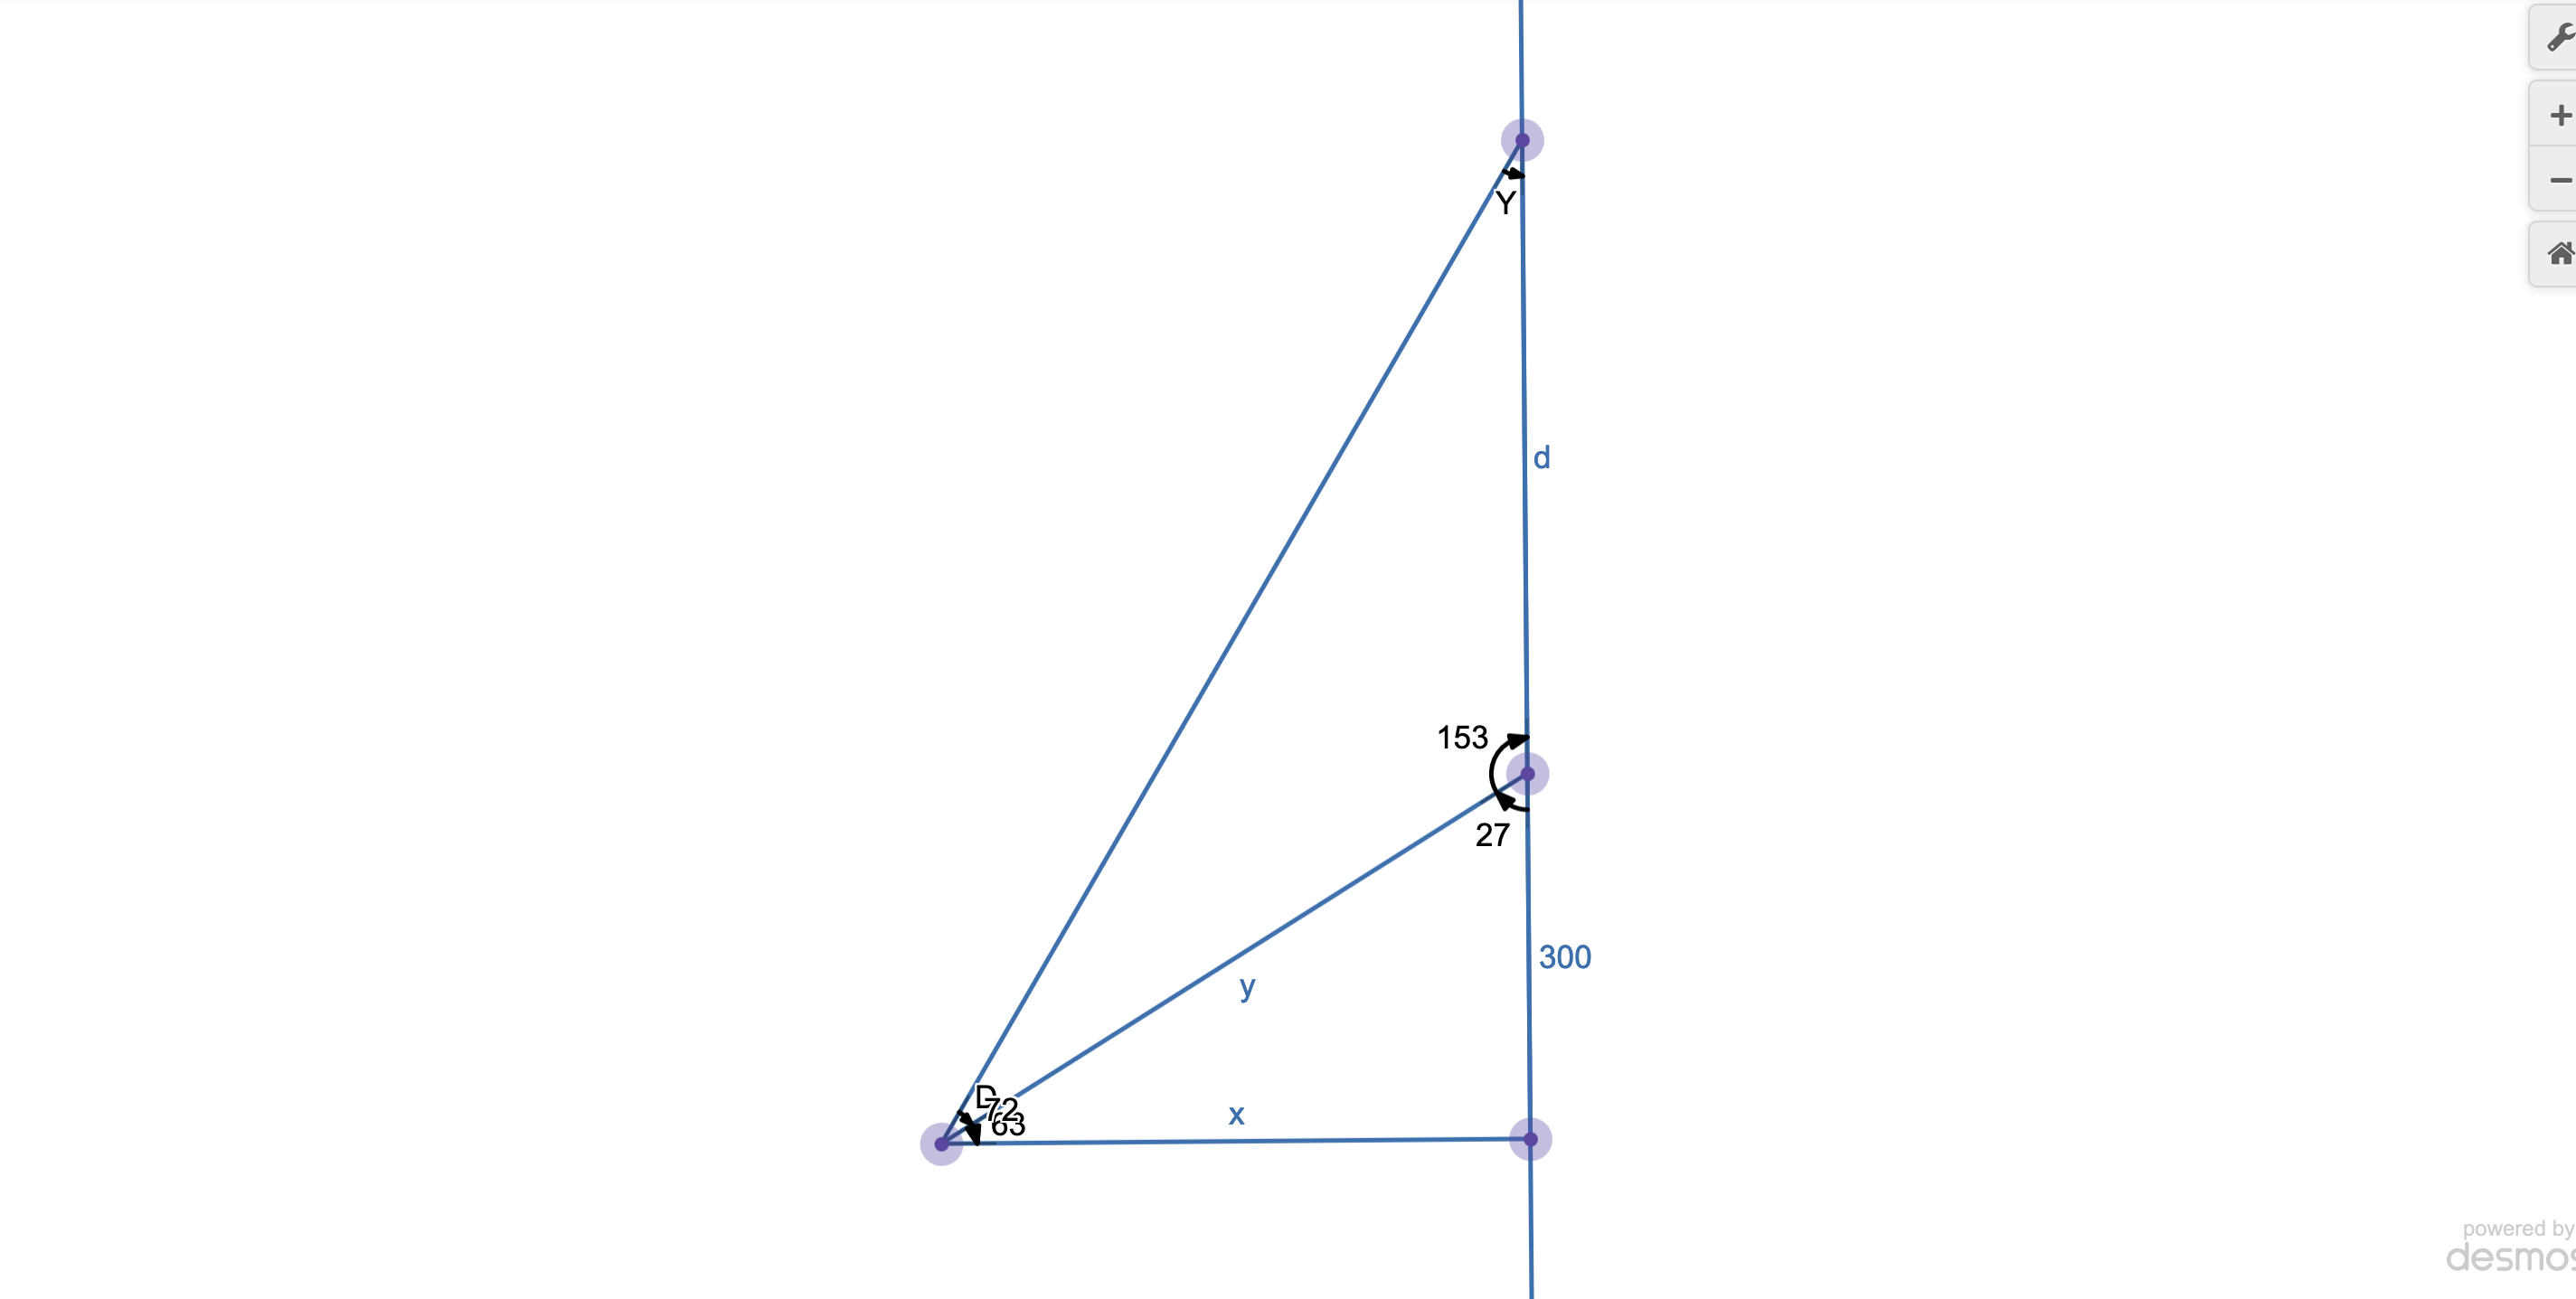
\includegraphics[width = 4in]{47} \newline 
The above diagram represents the given situation. $d$ is the height of the building. Having found $x$, there are two ways we can find $d$. The first is as follows: We know that 
\[ \tan 72^\circ=\frac{d+300}{x}=\frac{d+300}{152.86} \]
\[ d=152.86\tan 72^\circ-300 \]
\[ d\approx 170.45 \]
The second way is as follows: We can find $y$ by using the law of sines:
\[ \frac{300}{\sin 63^\circ}=\frac{y}{\sin 90^\circ} \]
\[ y\approx 336.70 \] 
We also know that $D=72-63=9^\circ$, meaning $Y=180-(9+153)=18^\circ$. Then we can use the law of sines again to find $d$:
\[ \frac{d}{\sin D}=\frac{y}{\sin Y} \]
\[ \frac{d}{\sin 9^\circ}=\frac{336.70}{\sin 18^\circ} \]
\[ d\approx 170.45 \] Thus we can conclude that the height of the building is about $170.45$ feet.

\section*{48}
(a): Suppose we have two lengths $8$ and $12$. Then the equation that gives the triangle's area $y$ as a function of $x$ is 
\[ y=\frac{1}{2}8\times 12\sin x \]
\[ y=48\sin x \] 

(b): \newline 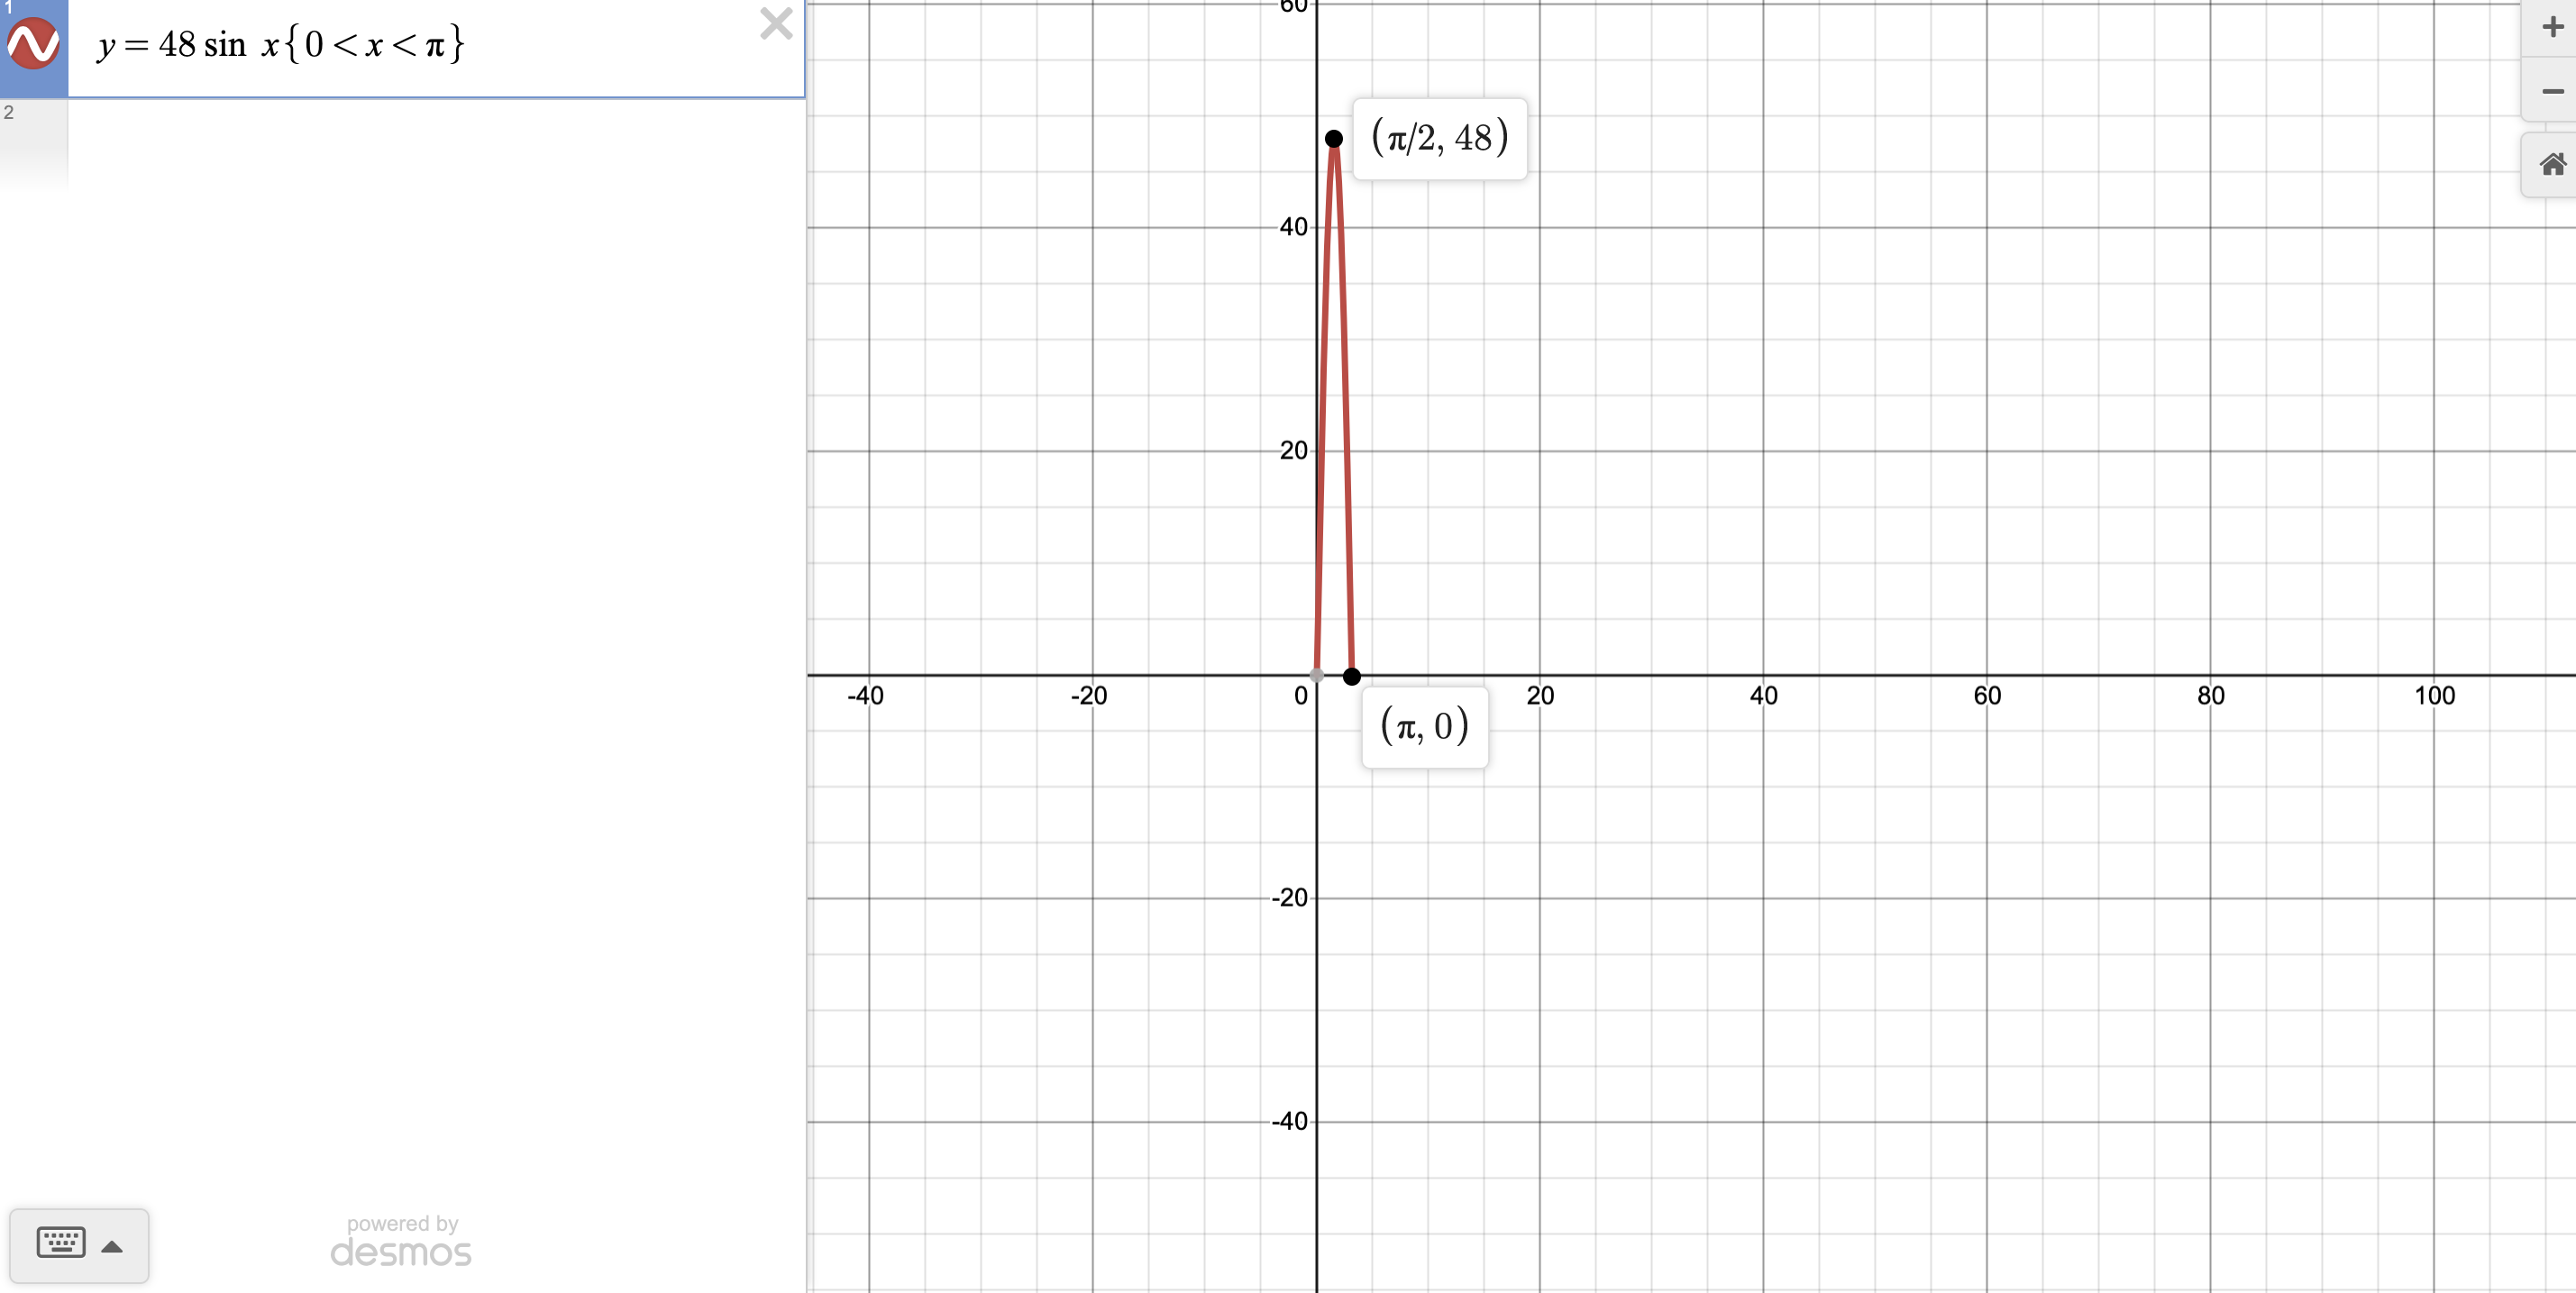
\includegraphics[width = 4in]{48}\newline 
From the graph, one can see that the area decreases from $\frac{\pi}{2}$ to $\pi$, meaning the area does not always increase as $x$ increases.


(c): The value of $x$ which maximizes the area of the triangle is $\frac{\pi}{2}$. Then the area is 48, which is equal to 
$\frac{1}{2}ab$ for the two sides $a$ and $b$ that were chosen in part (a).

\section*{49}
I was not sure how to solve this without using the law of cosines.

\end{document}
